\documentclass[tikz,border=3pt,10pt]{standalone}

\usepackage{fontspec}
\usepackage{unicode-math}
\usepackage{pgfplots}
\pgfplotsset{compat=1.18}

\setmainfont{STIXTwoText-Regular.otf}[
  Path=../../../../../../../assets/fonts/,
  BoldFont=STIXTwoText-Bold.otf,
  ItalicFont=STIXTwoText-Italic.otf,
  BoldItalicFont=STIXTwoText-BoldItalic.otf
]
\setmathfont{STIXTwoMath.otf}[Path=../../../../../../../assets/fonts/]
\usetikzlibrary{backgrounds}

% BEGIN ZO MATH GRAPH STYLE — VERSION 05 — 2026-07-30
% Copy this block verbatim into every graph source.
\definecolor{zoWhite}{HTML}{FFFFFF}
\definecolor{zoPlotBackground}{HTML}{FFF9E9}
\definecolor{zoPlotBorder}{HTML}{DFD7CA}
\definecolor{zoBackground}{HTML}{FBFAF8}
\definecolor{zoGridMinor}{HTML}{F8F5F0}
\definecolor{zoGridMajor}{HTML}{DFD7CA}
\definecolor{zoAxis}{HTML}{554F48}
\definecolor{zoText}{HTML}{3E3A35}
\definecolor{zoTextStrong}{HTML}{25221F}
\definecolor{zoGraphMain}{HTML}{EF5350}
\definecolor{zoGraphStrong}{HTML}{BF4240}
\definecolor{zoGraphSecondary}{HTML}{997918}
\definecolor{zoReference}{HTML}{997918}
\definecolor{zoHighlight}{HTML}{FFCA28}
\definecolor{zoHighlightLight}{HTML}{FFF4D4}
\definecolor{zoSuccess}{HTML}{1DE8B5}
\pgfplotsset{
  zo axis/.style={width=12cm,height=7.5cm,scale only axis,axis equal image=false,enlargelimits=false,clip=true,clip mode=individual,axis lines=middle,grid=none,axis line style={draw=zoAxis,line width=0.8pt,<->},tick align=center,tickwidth=0.4mm,tick style={draw=zoAxis,line width=0.32pt},every axis x label/.append style={text=zoText,font=\normalsize},every axis y label/.append style={text=zoText,font=\normalsize},every tick label/.append style={text=zoText,font=\footnotesize},every axis plot/.append style={line cap=round,line join=round}},
  zo grid/.style={major grid style={draw=zoGridMajor,line width=0.35pt},minor grid style={draw=zoGridMinor,line width=0.25pt}},
  zo graph main/.style={draw=zoGraphMain,line width=1.2pt,solid,no marks},
  zo graph secondary/.style={draw=zoGraphSecondary,line width=0.9pt,solid,no marks},
  zo graph strong/.style={draw=zoGraphStrong,line width=1.2pt,solid,no marks},
  zo reference/.style={draw=zoReference,line width=0.6pt,dashed,no marks},
  zo asymptote/.style={draw=zoReference,line width=0.8pt,dashed,no marks},
  zo auxiliary line/.style={draw=zoAxis,line width=0.6pt,densely dashed,no marks},
  zo point closed/.style={only marks,mark=*,mark size=2.2pt,draw=zoGraphMain,fill=zoGraphMain},
  zo point open/.style={only marks,mark=*,mark size=2.2pt,draw=zoGraphMain,fill=zoPlotBackground,line width=0.8pt},
  zo point emphasized/.style={only marks,mark=*,mark size=2.8pt,draw=zoGraphStrong,fill=zoGraphStrong},
  zo point auxiliary/.style={only marks,mark=*,mark size=1.7pt,draw=zoReference,fill=zoReference}
}
\tikzset{
  zo graph field/.style={show background rectangle,inner frame sep=4mm,background rectangle/.style={fill=zoPlotBackground,draw=zoPlotBorder,line width=0.45pt,rounded corners=2mm}},
  zo axis label/.style={text=zoText,font=\normalsize},zo origin label/.style={text=zoText,font=\normalsize},zo graph label/.style={text=zoText,font=\small},zo point label/.style={text=zoText,font=\small},zo tick label/.style={text=zoText,font=\footnotesize},zo reference label/.style={text=zoText,font=\small},zo legend label/.style={text=zoText,font=\small},zo auxiliary label/.style={text=zoText,font=\small}
}
% END ZO MATH GRAPH STYLE

\begin{document}
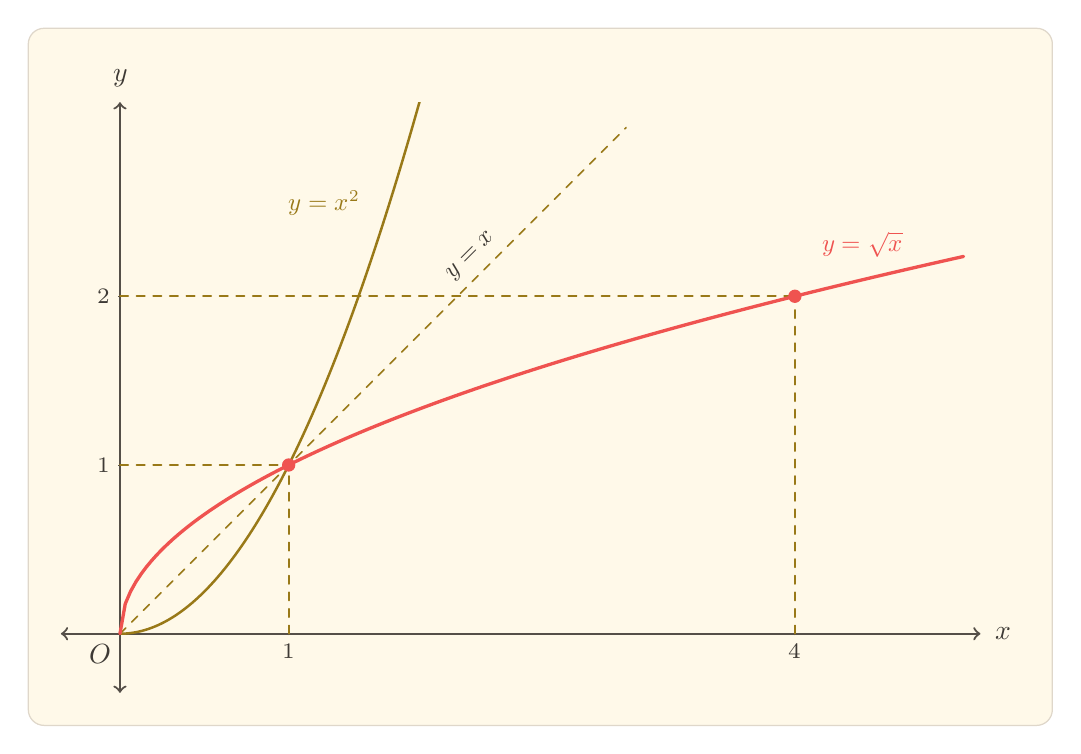
\begin{tikzpicture}[zo graph field]
  \begin{axis}[
    zo axis,
    axis equal image=true,
    xmin=-0.35,xmax=5.1,ymin=-0.35,ymax=3.15,
    xtick={1,4},xticklabel=\empty,
    ytick={1,2},yticklabel=\empty
  ]
    \addplot[zo reference] coordinates {(0,0) (3,3)}
      node[pos=0.72,above,sloped,zo reference label] {$y=x$};
    \addplot[zo reference] coordinates {(1,0) (1,1)};
    \addplot[zo reference] coordinates {(0,1) (1,1)};
    \addplot[zo reference] coordinates {(4,0) (4,2)};
    \addplot[zo reference] coordinates {(0,2) (4,2)};
    \addplot[zo graph secondary,domain=0:2.22,samples=120] {x^2};
    \addplot[zo graph main,domain=0:5,samples=160] {sqrt(x)};
    \addplot[zo point closed] coordinates {(1,1) (4,2)};
    \node[zo origin label,anchor=north east] at (axis cs:0,0) {$O$};
    \node[zo tick label,anchor=north] at (axis cs:1,0) {$1$};
    \node[zo tick label,anchor=east] at (axis cs:0,1) {$1$};
    \node[zo tick label,anchor=north] at (axis cs:4,0) {$4$};
    \node[zo tick label,anchor=east] at (axis cs:0,2) {$2$};
    \node[zo axis label,anchor=west,xshift=2pt] at (axis description cs:1,0.1) {$x$};
    \node[zo axis label,anchor=south,yshift=2pt] at (axis description cs:0.0642,1) {$y$};
    \node[zo graph label,anchor=south east,text=zoGraphMain] at (axis cs:4.7,2.17) {$y=\sqrt{x}$};
    \node[zo graph label,anchor=east,text=zoGraphSecondary] at (axis cs:1.48,2.55) {$y=x^2$};
  \end{axis}
\end{tikzpicture}
\end{document}
